\documentclass{article}
\usepackage{graphicx} % Required for inserting images
\usepackage{tabto}
\usepackage{amssymb}
\usepackage{amsthm}
\usepackage{tikz}
\usepackage{amsmath}
\usepackage{verbatim}
\usepackage{soul}
\usepackage{color}
\usepackage{float}
\usetikzlibrary{positioning}
\newcommand{\nl}{\nl}
\title{CISC 102 final project}
\author{David Balan}
\date{December 2023}

\begin{document}
\maketitle


\newpage
\section{Part 1: Topic Review}
\subsection{Sets And Logic}
\subsubsection{Topic: Intro to Truth Tables}

Creating truth tables is a method of comparing logical expressions. Logical expressions are made up of logical variables, often denoted by $p$, $q$, or $r$ or any other letter and hold the value \textbf{True}(1) or \textbf{False}(0). For every possible \textbf{True} and \textbf{False} value for a logical variable, there is a row on the truth table.

Logical operators include:
\begin{itemize}
  \item \textbf{Or} /($\vee$)– Returns \textbf{True} if one or two of the logical variables operated on are \textbf{True}. Otherwise, it returns \textbf{False}.

\begin{table}[ht]
    \centering
    \begin{tabular}{|l|c|c|} \hline 
          $p$&  $q$& $p\vee q$\\ \hline 
          0&  0& 0\\ \hline 
          0&  1& 1\\ \hline 
          1&  0& 1\\ \hline 
          1&  1& 1\\ \hline
    \end{tabular}
    \caption{Logical OR}
    \label{tab:my_label_one}
\end{table}
  \item \textbf{And}/($\wedge$) - Returns \textbf{True} if both of the logical variables operated on are \textbf{True}. Otherwise, it returns \textbf{False}.

\begin{table}[ht]
    \centering
    \begin{tabular}{|c|c|c|} \hline 
         $p$&  $q$& $p\wedge q$\\ \hline 
         0&  0& 0\\ \hline 
         0&  1& 0\\ \hline 
         1&  0& 0\\ \hline 
 1& 1&1\\ \hline
    \end{tabular}
    \caption{Logical AND}
    \label{tab:my_label_two}
\end{table}
  \item \textbf{Negate} – Changes the value of the logical variable to \textbf{False} if it is \textbf{True} and the reverse if it is already \textbf{False}.

\begin{table}[ht]
    \centering
    \begin{tabular}{|c|c|} \hline 
         $p$& $\neg p$\\ \hline 
         0& 1\\ \hline 
         1& 0\\ \hline
    \end{tabular}
    \caption{Logical Negation}
    \label{tab:my_label_three}
\end{table}

\end{itemize}

\subsubsection{Topic: Truth Tables and Their Properties}

Two logical expressions are logically equivalent if the result columns in their truth tables are the same. Some properties of logical expressions include:
\begin{itemize}
  \item \textbf{Associative property} – $((p \land q) \lor r)$ is equivalent to $(p \land (q \lor r))$. The order of evaluation does not matter.

  \item \textbf{Distributive Property} – When a logical expression is being operated on within another logical expression, you can expand the logical expression.
An example of this is $p\wedge(q\vee r) \equiv (p\wedge q)\vee(p \wedge r)\\$
This can be proved with a truth table:

\begin{table}[ht]
    \centering
    \begin{tabular}{|c|c|c|c|c|c|c|c|} \hline 
         $p$&  $q$&  $r$&  $q \vee r$&  $p \wedge (q\vee r)$&  $p \wedge q$&  $p \wedge r$& $(p\wedge q)\vee(p \wedge r)$\\ \hline 
         0&  0&  0&  0&  0&  0&  0& 0\\ \hline 
         0&  0&  1&  1&  0&  0&  0& 0\\ \hline 
         0&  1&  0&  1&  0&  0&  0& 0\\ \hline 
         0&  1&  1&  1&  0&  0&  0& 0\\ \hline 
         1&  0&  0&  0&  0&  0&  0& 0\\ \hline 
         1&  0&  1&  1&  1&  0&  1& 1\\ \hline 
         1&  1&  0&  1&  1&  1&  0& 1\\ \hline 
         1&  1&  1&  1&  1&  1&  1& 1\\ \hline
    \end{tabular}
    \caption{Proving that $p\wedge(q\vee r) \equiv (p\wedge q)\vee r$}
    \label{tab:my_label_four}
\end{table}

  \item \textbf{DeMorgan’s Law} – The distribution of the negate operation changes the logical expression by changing the logical operator or to and as and changes the logical variable to the opposite \textbf{True} or \textbf{False} value.
$\neg(p\wedge q) \equiv \neg p \vee \neg q \\$
$\neg(p\vee q) \equiv \neg p \wedge \neg q\\$
\end{itemize}

\subsubsection{Topic: Intro to Set Theory}

Set theory is the logical-mathematical study of sets. A set is an unordered collection of objects called elements. Sets can be finite or infinite and may sometimes contain duplicates. These sets are often used when trying to state the domain or range of a function. For example, in the domain of a reciprocal function $1/x$, $x$ is an element of all real numbers such that $x$ is not equal to zero. Sometimes it is written as such:
$D: \{ x \in \mathbb{R} | x \not = 0 \} \\$
Similar to simple mathematics, sets can also have operations performed on them such as union, intersection, difference, and complement.

\begin{itemize}
  \item \textbf{Union} – Represents all of the elements contained in both sets A and B combined and shown by $A \cup B.\\$
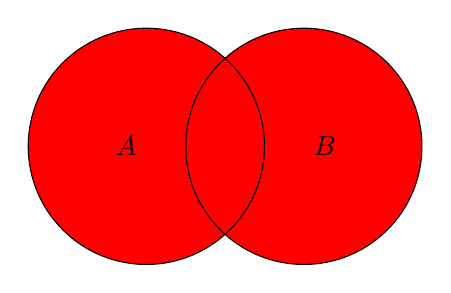
\begin{tikzpicture}
  % Set A
  \begin{scope}[even odd rule]
    \clip (0,0) circle (1.5);
    \fill[red] (0,0) circle (1.5);
  \end{scope}

  % Set B
  \begin{scope}[even odd rule]
    \clip (2,0) circle (1.5);
    \fill[red] (2,0) circle (1.5);
  \end{scope}

  % Union of A and B
  \begin{scope}
    \clip (0,0) circle (1.5);
    \clip (2,0) circle (1.5);
    \fill[red] (0,0) circle (1.5);
  \end{scope}

  % Draw circles
  \draw (0,0) circle (1.5) node[left] {$A$};
  \draw (2,0) circle (1.5) node[right] {$B$};
\end{tikzpicture}

  \item \textbf{Intersect} – This represents all of the matching elements in both sets A and B. Shown by $A \cap B.\\$
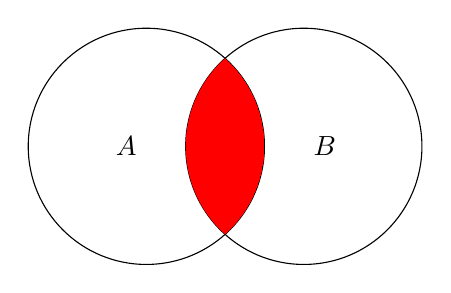
\begin{tikzpicture}
  % Set A
  \draw (0,0) circle (1.5) node[left] {$A$};
  % Set B
  \draw (2,0) circle (1.5) node[right] {$B$};

  % Intersection of A and B
  \begin{scope}
    \clip (0,0) circle (1.5);
    \clip (2,0) circle (1.5);
    \fill[red] (0,0) circle (1.5);
  \end{scope}
\end{tikzpicture}
  \item \textbf{Set Difference} – This represents all of the elements of A which are not also contained in set B.$\\$
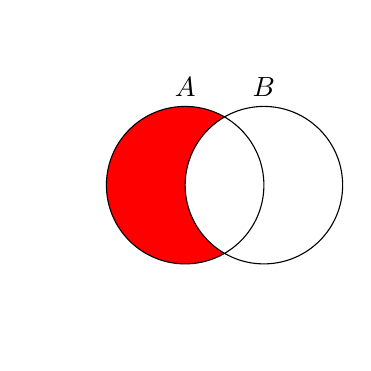
\begin{tikzpicture}[fill=red]
% left hand
\scope
\clip (-2,-2) rectangle (2,2)
      (1,0) circle (1);
\fill (0,0) circle (1);
\endscope
% right hand
% outline
\draw (0,0) circle (1) (0,1)  node [text=black,above] {$A$}
      (1,0) circle (1) (1,1)  node [text=black,above] {$B$};
\end{tikzpicture}
  \item \textbf{Complement} – The complements represent all of the elements which are not in A.$\\$
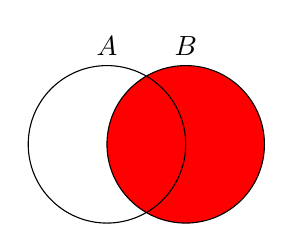
\begin{tikzpicture}[fill=red]
% right hand
\scope
\fill (1,0) circle (1);
\endscope
% outline
\draw (0,0) circle (1) (0,1)  node [text=black,above] {$A$}
      (1,0) circle (1) (1,1)  node [text=black,above] {$B$};
\end{tikzpicture}
  \item \textbf{Subsets} – $A$ is a subset of $B$ if all of the elements of $A$ are also in $B$. $A$ is a proper subset of $B$ when $A$ is not equal to $B$.
\end{itemize}

\subsubsection{Topic: Power Sets}

Some of the properties of sets are different from the properties of logical expressions:

\begin{itemize}
  \item \textbf{DeMorgan’s Law} - The negate operator makes a set into a complement. This means the set becomes a set of all elements in the universal set which are not in the current set.

\noindent
\item \textbf{Power Set:} The power set is the set of all subsets of a specified set. Sets within a set are considered an element of the specific set.

\noindent
\item \textbf{Indexed Set:} An indexed set is a set described by a formula for the '$i$' index. The letter '$i$' represents an integer. Set operations can be performed on the index to show that the set is made up of changed integer values.
\end{itemize}
\subsubsection{Topic: Set Equality}

Two sets are equal whenever each set is a subset of each other. You can prove this by showing any arbitrary element of set $A$ is an element of the set $B$ and any arbitrary element of the set $B$ is an element of set $A$.

\subsubsection{Topic: Set Equality - Principles of Inclusion and Exclusion}

The cardinality of a set is $|A|$, the count of the number of elements of the set. This is similar to finding the length of an array or a list in computer science

For example: $|A \cup B| = |A| + |B| - |A \cap B|$

The non-repeating union of two sets is equal to the two sets added together subtract the intersection of $A$ and $B$.

\fbox{
    \parbox{\linewidth}{
        \textbf{Helpful Reminders:}
        \begin{itemize}
            \item Creating truth tables is a useful method in comparing logical expressions
            \item Logical expressions are made up of logical variables, often denoted by $p$, $q$, or $r$, and hold the value \textbf{True} (1) or \textbf{False} (0)
            \item \textbf{Or} – Returns \textbf{True} if one or two of the logical variables operated on are \textbf{True}. Otherwise, it returns \textbf{False}.
            \item \textbf{And} - Returns \textbf{True} if both of the logical variables operated on are \textbf{True}. Otherwise, it returns \textbf{False}.
            \item \textbf{Negate} – Changes the value of the logical variable to \textbf{False} if it is \textbf{True} and the reverse if it is already \textbf{False}.
            \item \textbf{Associative property} – $((p \land q) \lor r)$ is equivalent to $(p \land (q \lor r))$. The order of evaluation does not matter.
            \item \textbf{Distributive Property} – When a logical expression is being operated on within another logical expression, you can expand the logical expression.
            \item \textbf{DeMorgan’s Law} – The distribution of the negate operation changes the logical expression.
        \end{itemize}
    }
}

\subsection{Properties Of Integers}
\subsubsection{Topic: Proofs}

All logical proofs follow the same basic format: 
$$\textrm{"If x then y”, meaning that if x is true, then y must be true}
(x \rightarrow y)$$
A bi-conditional implies $x$ if and only if $y$
\begin{center}
This means that the statement is true only when x and y have the same value
$(x \leftrightarrow y)$.
\end{center}
 Converse is used when some logical implication
 \begin{center}
    $ x \rightarrow y$ is $y \leftarrow x$. \\ For the logical implication $x \rightarrow y$, it is equivalent to $\neg x \rightarrow \neg y$.
 \end{center} This is called the contra-positive.
\\\\
There are also several quantifiers:
\begin{itemize}
    \item $\exists$ translates to "there exists". This means that there will be a value that will satisfy a condition. It is also known as the existential quantifier. 
    \item The universal quantifier can be written as "$\forall$". It is also known as "for all" and it means that every possible element in the universal set will satisfy the condition.
\end{itemize}

The goal of a proof is to get from point A to B using logical arguments. Many different proof methods can be used:
\begin{itemize}
    \item \textbf{Direct Proof:} "If A then B"
\end{itemize}
There are also indirect proofs that can be used to get from point A
to B
\begin{itemize}
    \item \textbf{Contrapositive:} "If \underline{Not B} then Not A"
    \item \textbf{Contradiction:} In this method, assume that A is true
    and B is false. Afterwards, apply theorems and definitions, and
    arithmetic until a contradiction occurs.
\end{itemize}


\subsubsection{Topic: Integer Properties}
\textbf{Divisibility} is also used for proofs. For example, a divides b(a$\mid$b) if and only if some element m is an integer such that a$\cdot$m = b.
\\\textbf{A prime} number is when a$\mid$b results in a = 1 or a = b. If an integer
is not prime it is composite. The fundamental theorem of arithmetic
states that any integer n, can be written as a unique product of primes. \\ \textbf{he greatest common divisor}(GCD(a,b)) is the largest integer
that divides both a and b. \\\textbf{The least common multiple}(LCM(a,b)) is the
smallest integer that divides both a and b. \\\textbf{Modulo}  is an operation that gives the remainder when a is divided by b and some integer
\begin{itemize}
    \item \textbf{Fundamental Theorem of Arithmetic} n = $P_1^{r_1}$ $P_2^{r_2}$...$P_k^{r_k}$
    \item \textbf{Euclidean Algorithm} a = bq + r
\end{itemize}



\newpage
\fbox{
  \parbox{\linewidth}{
    \textbf{Helpful Reminders:}

    \begin{itemize}
      \item \textbf{Logical Proofs:}
        \begin{itemize}
          \item Basics: Understand "if \(x\) then \(y\)" (\(x \rightarrow y\)) and bi-conditionals (\(x \leftrightarrow y\)).
          \item Converse: Recognize the use of the converse in logical implications.
          \item Quantifiers: \(\exists\) means "there exists," and \(\forall\) means "for all" in set conditions.
        \end{itemize}
      
      \item \textbf{Proof Construction:}
        \begin{itemize}
          \item Direct Proof: Follow the logic of "If A then B."
          \item Indirect Proofs: Consider methods like contrapositive and contradiction.
        \end{itemize}
      
      \item \textbf{Integer Properties:}
        \begin{itemize}
          \item Divisibility: \(a\) divides \(b\) (\(a \mid b\)) if some integer \(m\) satisfies \(am = b\).
          \item Primality: An integer \(a\) is prime if \(a \mid b\) results in \(a = 1\) or \(a = b\).
          \item Composite Numbers: Non-prime integers are composite.
          \item Fundamental Theorem of Arithmetic: Any integer \(n\) is a unique product of primes.
          \item GCD and LCM: Understand the concepts of the greatest common divisor (GCD) and least common multiple (LCM).
          \item Modulo: Remember that modulo provides the remainder when \(a\) is divided by \(b\).
        \end{itemize}
    \end{itemize}
  }
}


\newpage
\subsection{Counting}

\subsubsection{Topic: Introduction to Counting}
\begin{itemize}
    \item \textbf{Replacement}: if an object can be counted again, we say it has "Replacement"\\
    e.g., How many possible 4-digit passwords?
    \item \textbf{Permutations}: When the order of the "n" counted objects matter, each successive multiplication of n will be 1 less. We use factorials to count permutations.\\
    (e.g., How many ways to give 5 friends a banana from 23 bananas?)
    \textbf{Combinations}: When the order of the $n$ counted objects does not matter $\binom{n}{k}$ or $\frac{n!}{k!(n-k)!}$ counts $k$ objects out of the $n$ without replacement.

\end{itemize}

\begin{table}[ht]
    \centering
    \begin{tabular}{c|cc}
                    &  Replacement& No repetition\\
    \hline Order      &  $n^{k}$& $_{n}P_{k}$\\
         No Order   &  & $_{n}C_{k}$\\
    \end{tabular}
    \caption{Ways to count "n" objects}
\end{table}

\subsubsection{Topic: Principle of Inclusion and Exclusion for Counting}
Recalling from past units that $|A\cup B| = |A|+|B|-|A\cap B|$:
\\

E.g. A large software development company employs 100 computer programmers. Of them, 45 are proficient in Java, 30 in C\#, 20 in Python, six in C\# and Java, one in Java and Python, five in C\# and Python, and just one programmer is proficient in all three languages above.\\
Let $U$ denote the set of all employed computer programmers and let $J$, $C$ and $P$ denote the set of programmers proficient in Java, C\# and Python, respectively. Thus:
$\\|U| = 100\\$
$|J| = 45\\$
$|C| = 30\\$
$|P| = 20\\$
$|J \cap C| = 6\\$
$|J \cap P| = 1\\$
$|C \cap P| = 5\\$
$|J \cap C \cap P| = 1\\$
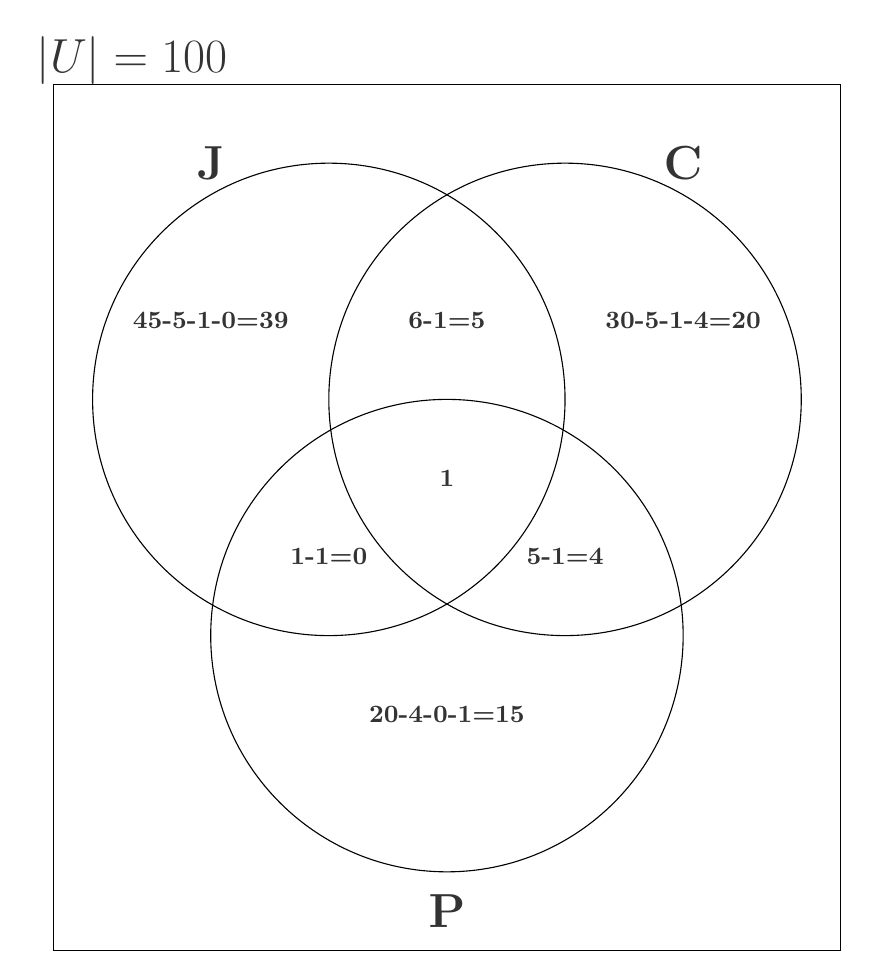
\begin{tikzpicture}
    \centering
    \begin{scope} [fill opacity = .8]
        \draw (-5,5) rectangle (5,-6);
        \draw[draw = black] (-1.5,1) circle (3);
        \draw[draw = black] (1.5,1) circle (3);
        \draw[draw = black] (0,-2) circle (3);
        \node at (-4,5.3) {\LARGE\textbf{$|U| = 100$}};
        \node at (-3,4) {\LARGE\textbf{J}};
        \node at (3,4) {\LARGE\textbf{C}};
        \node at (0,-5.5) {\LARGE\textbf{P}};
        \node at (-3,2) {\small\textbf{45-5-1-0=39}};
        \node at (0,2) {\small\textbf{6-1=5}};
        \node at (3,2) {\small\textbf{30-5-1-4=20}};
        \node at (0,0) {\small\textbf{1}};
        \node at (0,-3) {\small\textbf{20-4-0-1=15}};
        \node at (-1.5,-1) {\small\textbf{1-1=0}};
        \node at (1.5,-1) {\small\textbf{5-1=4}};
    \end{scope}
\end{tikzpicture}
$\\$We know that if $|U|=100$ \& $|J \cup C \cup P|=84$ then $\\\overline{|J \cup C \cup P|} \\= |U| - |J \cup C \cup P| \\= 100 - 84 = 16$



\subsubsection{Topic: Pigeonhole Principle}
The Pigeonhole Principle allows us to logically prove a statement is true by demonstrating that if n elements (pigeons) are put into m sets (containers) such that $n > m$, then there will be a set (container) with more than 1 element (pigeon).\\

\subsubsection{Topic: Pascal's Triangle}
Pascal's Triangle is a pyramid arrangement of numbers. Every number in the triangle is obtained by adding the two numbers directly above it. Every $n$ row of Pascal's Triangle gives the binomial coefficients of $(x+y)^n$. Pascal's Triangle is also useful for evaluating combinations. For example, $3\choose2$ can be found as the 2nd term of the 3rd row (counting from the 0th row and 0th term). Additionally, the Pascal Triangle is used for questions such as counting the number of lattice paths from point A to B. 

\begin{table}[ht]
    \centering
    \begin{tabular}{ccccccccc}
          &&  &  &  1&  &  &  &\\
          &&  &  1&  &  1&  &  &\\
          &&  1&  &  2&  &  1&  &\\
          &1&  &  3&  &  3&  & 1&\\
          1&&  4&  &  6&  &  4&  &1\\
    \end{tabular}
    \caption{Pascal's Triangle up to the 4th Row}
    \label{tab:my_label_five}
\end{table}
\begin{table}[ht]
    \centering
    \begin{tabular}{ccccccccc}
          &&  &  &  $0\choose0$&  &  &  &\\
          &&  &  $1\choose0$&  &  $1\choose1$&  &  &\\
          &&  $2\choose0$&  &  $2\choose1$&  &  $2\choose2$&  &\\
          &$3\choose0$&  &  $3\choose1$&  &  $3\choose2$&  & $3\choose3$&\\
          $4\choose0$&&  $4\choose1$&  &  $4\choose2$&  &  $4\choose3$&  &$4\choose4$\\
    \end{tabular}
    \caption{Pascal's Triangle represented in Choose notation}
    \label{tab:my_label_six}
\end{table}


\textbf{Counting With Repetition:} In a given counting problem, If we can choose the same object again \\
e.g.: There are 3 unique balls in a bag how many combinations of 3 is there if you put the ball back every time\\
\\
\textbf{Counting Without Repetition: }In a given counting problem, if we cannot choose the same object again.\\
e.g.: there are three unique balls in a bag, how many combinations of 3 are there if you do not replace the ball after choosing it \\
\textbf{Factorial}$(!)$: $n!=n\cdot (n-1) \cdot (n-2) \cdot \ldots \cdots (1)$

\newpage
\fbox{
\parbox{\textwidth}{
\textbf{Helpful Reminders:}
\begin{itemize}
    \item \textbf{Replacement:} Objects can be counted again.
    \item \textbf{Permutations:} Order matters, and factorials are used.
    \item \textbf{Combinations:} Order doesn't matter, and \(nCk\) counts combinations without replacement.
\end{itemize}

\textbf{Principle of Inclusion and Exclusion for Counting}
Utilizes the formula \(\lvert A \cup B \rvert = \lvert A \rvert + \lvert B \rvert - \lvert A \cap B \rvert\) for counting. Demonstrated in an example involving drawing marbles from a bag.

\textbf{Pigeonhole Principle}
Logical proof method stating that if \(n\) elements are put into \(m\) sets (\(n > m\)), then there will be a set with more than one element.

\textbf{Pascal's Triangle}
Pyramid arrangement of numbers. Used to find binomial coefficients and evaluate combinations. Helpful for problems like counting lattice paths.
}} \newpage


\subsection{Functions and Relations}

\subsubsection{Topic: Summation}
\textbf{Summation:} An expression with the 
form: \\
$\sum_{i=0}^{n} f(x)=f(0)+f(1)...+f(n)$ \newline

\subsubsection{Topic: Proofs By Induction}
\textbf{Proof By Induction:} A way to prove an equality, generally when there is a summation on one side of it, in three steps:

\begin{enumerate}
  \item \textbf{Base Case:} Show that the statement holds true for the base case, usually when \(n = 1\) or \(n = 0\).
  \item \textbf{Inductive Step:} Prove that if the statement is true for \(k\), then it must also be true for \(k + 1\). This often involves using the assumption from the inductive hypothesis to prove \(P(k+1)\).
\end{enumerate}

\begin{flushleft}
By completing these steps, you establish that the statement holds for all positive integers \(n\) by induction.
\end{flushleft}
\subsubsection{Topic: Series}
\begin{flushleft}
\textbf{Arithmetic Series:} A series that starts with $a_0$ and increments by $d$ for each occurrence. It has a closed form and a recursive definition:
\end{flushleft}
\begin{itemize}
  \item \textbf{Recursive Definition:} \(a_n = a_{n-1} + d\)
  \item \textbf{Closed Form:} \(a_n = a_0 + nd\)
\end{itemize}
\begin{flushleft}
\textbf{Geometric Series:} A series that starts with $a_0$ and multiplies by $r$ for $n$ times. It also has a closed and recursive form:
\end{flushleft}
\begin{itemize}
  \item \textbf{Recursive Definition:} \(a_n = a_{n-1} \cdot r\)
  \item \textbf{Closed Form:} \(a_n = a_0 \cdot r^n\)
\end{itemize}
\begin{flushleft}
\subsubsection{Topic: Relations and Their Properties}
\textbf{Binary Relation:} $aRb$ on set A relates the two elements a and b.
\end{flushleft}
$R(\text{Relation}) = \{(a, b) \, \text{S.T.} \, a, b \in A \mid aRb\}$

\begin{flushleft}
\textbf{Properties of Relations:} 
\end{flushleft}
\begin{itemize}
  \item \textbf{Reflexive:} R is reflexive if every element in set A can relate to itself. That is to say R is reflexive if 
  \begin{center}
$(a,a) \in R, \forall a \in a$
\end{center}
  \item \textbf{Symmetric:} R is reflexive if 
 \begin{center} in $(a,b), \, aRb$ and $bRa$. \end{center}
  \item \textbf{Transitive:} R is transitive if for a,b,c in set A with $aRb$ and $bRc$ then $aRc$, that is to say, R is Transitive if:
  \begin{center} in $aRb$ and $bRc$ then $aRc$ \end{center}
  \item \textbf{Ir-reflexive:}  R is irreflexive if $xRx$ does not hold for any $x$ in a set $A$, that is to say $R$ is irreflexive if:
  \begin{center} $\forall a \in A$,  $\neg (aRa)$ \end{center}
  
  \item \textbf{Anti-symmetric:} R is anti-symmetric if 
   \begin{center} $aRb$ and $bRa$ and $a=b$ \end{center}
\end{itemize}
\begin{flushleft}
\textbf{Types of Relations:} 
\end{flushleft}
\begin{itemize}
  \item \textbf{Equivalence Relation:} R is an equivalence relation if it is reflexive, symmetric and transitive.
  \item \textbf{Partial Order:}  R is a partial order if a relation is reflexive, anti-symmetric and transitive
\end{itemize}
\subsubsection{Topic: Functions}
\textbf{Function:} A relation is a function if every x has 1 unique y value such that $f(x)$ holds. We also write functions in the form $f:x \rightarrow y$.
\begin{flushleft}
\textbf{Properties of Functions:} 
\end{flushleft}
\begin{itemize}
\item \textbf{One to One/Injective:}  A function is one-to-one if no y values are repeated, each unique x has a unique y. That is to say $f:x \rightarrow y$ is one-to-one if:
\begin{center}$f(x_{1})=f(x_{2})$ for some $x_{1},x_{2}$.\end{center}

\item \textbf{Onto/Surjective:} A function is onto if for every y there exists an x which can map to it. That is to say $f:x \rightarrow y$ is onto if:

\begin{center} for every $y$, their exists some $x \, S.T f(y) = x$ \end{center}
\item \textbf{Bijection:} A function is a bijection if it is one-to-one and onto.
\end{itemize}
\subsubsection{Topic: Hasse Diagrams}
\textbf{Hasse Diagram:} A diagram which demonstrates a set, usually a finite partial order with nodes and lines. The following Hasse diagram shows the relation $A=(x)$, $B=(y)$, $ARB$
\begin{center} 
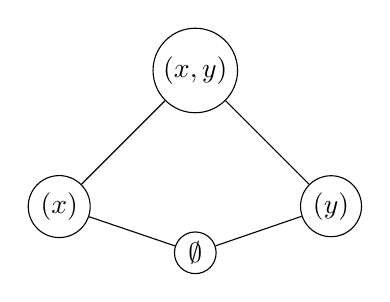
\begin{tikzpicture}[node distance=1.5cm, every node/.style={draw, circle, inner sep=2pt}]

  \node (xy) {$(x, y)$};
  \node[below left=of xy] (x) {$(x)$};
  \node[below right=of xy] (y) {$(y)$};
  \node[below=of xy] (empty) {$\emptyset$};

  \draw (xy) -- (x);
  \draw (xy) -- (y);
  \draw (x) -- (empty);
  \draw (y) -- (empty);

\end{tikzpicture}
\end{center}


\fbox{\parbox{\textwidth}{
\textbf{Some Helpful Reminders}

\begin{itemize}
  \item \textbf{Functions and Relations:}
    \begin{itemize}
      \item Understand summation notation for adding function values.
      \item Follow the steps of proof by induction: Base Case and Inductive Step.
    \end{itemize}

  \item \textbf{Series:}
    \begin{itemize}
      \item Distinguish arithmetic and geometric series.
      \item Recognize the recursive and closed-form definitions for each series.
    \end{itemize}

  \item \textbf{Relations and Properties:}
    \begin{itemize}
      \item Know the properties of binary relations: Reflexive, Symmetric, Transitive, Ir-reflexive, Anti-symmetric.
      \item Differentiate between Equivalence Relations and Partial Orders.
    \end{itemize}

  \item \textbf{Functions:}
    \begin{itemize}
      \item Identify a function by its unique mapping of \(x\) to \(y\).
      \item Understand properties like injective, surjective, and bijective functions.
    \end{itemize}

  \item \textbf{Hasse Diagrams:}
    \begin{itemize}
      \item Visualize finite partial orders using Hasse diagrams.
    \end{itemize}

  \item \textbf{Reminders:}
    \begin{itemize}
      \item Focus on the base case and inductive step in mathematical induction.
      \item Differentiate between arithmetic and geometric series.
      \item Be aware of the properties of relations and their distinctions.
      \item Understand the characteristics of functions: injective, surjective, and bijective.
      \item Interpret Hasse diagrams with nodes representing elements and lines indicating relations.
    \end{itemize}
\end{itemize}
}}\newpage



\section{Part 2: Problem Set}
\subsection{Sets and Logic}
\subsubsection{Q1}
$\\$(a) Let $A$, $B$, $C$ be sets such that $|A| = x$, $|B| = y$, $|C| = z$. Determine exactly or state a range of values:
(i)$|A \cup B|$
    \[
    |A \cup B| = |A| + |B| - |A \cap B|
    \]
    \[
    = x + y - |A \cap B|
    \]

    The range of values is:
    \[
    x + y \leq |A \cup B| \leq \max(x, y)
    \]
(ii)$|C \setminus (A \cup B)|$
    \[
    |C \setminus (A \cup B)| = |C| - |A \cup B|
    \]
    \[
    = |C| - (|A| + |B| - |A \cap B|)
    \]
    \[
    = |C| - (x + y - |A \cap B|)
    \]

    The range of values is:
    \[
    0 \leq |C \setminus (A \cup B)| \leq z
    \]
(b)Let $U = \{1, 2, 3, 4, 5\}$, $A = \{1, 2, 3\}$, and $B = \{2, 3, 4\}$. List the elements of the following:
(i) $(A \times B) \cup (A \times A)$
\[
(A \times B) \cup (A \times A)\] \newline  $= \{(1,2), (1,3), (1,4), (2,2), (2,3), (2,4), (3,2), (3,3), (3,4)\}\newline \cup
\{(1,1), (1,2), (1,3), (2,1), (2,2), (2,3), (3,1), (3,2), (3,3)\}$
\[
= \{(1,1), (1,2), (1,3), (1,4), (2,1), (2,2), (2,3), (2,4), (3,1), (3,2), (3,3), (3,4)\}
\]
(ii) $B \times (A \setminus B)$
\[
B \times (A \setminus B) = \{2, 3, 4\} \times \{1\}
\]

\[
= \{(2, 1), (3, 1), (4, 1)\}
\]
(iii) \(\overline{B}\)

$\overline{B} = \{1, 5\}$
\subsubsection{Q2}
Use a truth table to show that
    \[((p \rightarrow q) \land \lnot q) \rightarrow ((r \rightarrow q) \rightarrow r) \equiv (p \lor q) \lor (r \land (\lnot q \lor r))\]
    We will take the left side and right side and compare the answers. If they are identical then we have proved the equivalence.
$\\L.S.:\\$
\begin{tabular}{@{ }c@{ }@{ }c@{ }@{ }c | c@{ }@{}c@{}@{}c@{}@{ }c@{ }@{ }c@{ }@{ }c@{ }@{}c@{}@{ }c@{ }@{ }c@{ }@{ }c@{ }@{}c@{}@{ }c@{ }@{}c@{}@{}c@{}@{ }c@{ }@{ }c@{ }@{ }c@{ }@{}c@{}@{ }c@{ }@{ }c@{ }@{}c@{}@{ }c}
p & q & r &  & ( & ( & p & $\rightarrow$ & q & ) & $\land$ & $\lnot$ & q & ) & $\rightarrow$ & ( & ( & r & $\rightarrow$ & q & ) & $\rightarrow$ & r & ) & \\
\hline 
1 & 1 & 1 &  &  &  & 1 & 1 & 1 &  & 0 & 0 & 1 &  & \textcolor{red}{1} &  &  & 1 & 1 & 1 &  & 1 & 1 &  & \\
1 & 1 & 0 &  &  &  & 1 & 1 & 1 &  & 0 & 0 & 1 &  & \textcolor{red}{1} &  &  & 0 & 1 & 1 &  & 0 & 0 &  & \\
1 & 0 & 1 &  &  &  & 1 & 0 & 0 &  & 0 & 1 & 0 &  & \textcolor{red}{1} &  &  & 1 & 0 & 0 &  & 1 & 1 &  & \\
1 & 0 & 0 &  &  &  & 1 & 0 & 0 &  & 0 & 1 & 0 &  & \textcolor{red}{1} &  &  & 0 & 1 & 0 &  & 0 & 0 &  & \\
0 & 1 & 1 &  &  &  & 0 & 1 & 1 &  & 0 & 0 & 1 &  & \textcolor{red}{1} &  &  & 1 & 1 & 1 &  & 1 & 1 &  & \\
0 & 1 & 0 &  &  &  & 0 & 1 & 1 &  & 0 & 0 & 1 &  & \textcolor{red}{1} &  &  & 0 & 1 & 1 &  & 0 & 0 &  & \\
0 & 0 & 1 &  &  &  & 0 & 1 & 0 &  & 1 & 1 & 0 &  & \textcolor{red}{1} &  &  & 1 & 0 & 0 &  & 1 & 1 &  & \\
0 & 0 & 0 &  &  &  & 0 & 1 & 0 &  & 1 & 1 & 0 &  & \textcolor{red}{0} &  &  & 0 & 1 & 0 &  & 0 & 0 &  & \\
\end{tabular}
$\\R.S.:\\$
\begin{tabular}{@{ }c@{ }@{ }c@{ }@{ }c | c@{ }@{}c@{}@{ }c@{ }@{ }c@{ }@{ }c@{ }@{}c@{}@{ }c@{ }@{}c@{}@{ }c@{ }@{ }c@{ }@{}c@{}@{ }c@{ }@{ }c@{ }@{ }c@{ }@{ }c@{ }@{}c@{}@{}c@{}@{ }c}
p & q & r &  & ( & p & $\lor$ & q & ) & $\lor$ & ( & r & $\land$ & ( & $\lnot$ & q & $\lor$ & r & ) & ) & \\
\hline 
1 & 1 & 1 &  &  & 1 & 1 & 1 &  & \textcolor{red}{1} &  & 1 & 1 &  & 0 & 1 & 1 & 1 &  &  & \\
1 & 1 & 0 &  &  & 1 & 1 & 1 &  & \textcolor{red}{1} &  & 0 & 0 &  & 0 & 1 & 0 & 0 &  &  & \\
1 & 0 & 1 &  &  & 1 & 1 & 0 &  & \textcolor{red}{1} &  & 1 & 1 &  & 1 & 0 & 1 & 1 &  &  & \\
1 & 0 & 0 &  &  & 1 & 1 & 0 &  & \textcolor{red}{1} &  & 0 & 0 &  & 1 & 0 & 1 & 0 &  &  & \\
0 & 1 & 1 &  &  & 0 & 1 & 1 &  & \textcolor{red}{1} &  & 1 & 1 &  & 0 & 1 & 1 & 1 &  &  & \\
0 & 1 & 0 &  &  & 0 & 1 & 1 &  & \textcolor{red}{1} &  & 0 & 0 &  & 0 & 1 & 0 & 0 &  &  & \\
0 & 0 & 1 &  &  & 0 & 0 & 0 &  & \textcolor{red}{1} &  & 1 & 1 &  & 1 & 0 & 1 & 1 &  &  & \\
0 & 0 & 0 &  &  & 0 & 0 & 0 &  & \textcolor{red}{0} &  & 0 & 0 &  & 1 & 0 & 1 & 0 &  &  & \\
\end{tabular} \newline
Since the final column of each chart is equal, we have proven the equivalence
$\\\therefore$ The equivalence has been proved as true. 

\subsubsection{Q3}
\subsubsection{Q4}
Let $X = \{x \in \mathbb{Z} \mid 3 \mid x\}$ and $Y = \{y \in \mathbb{Z} \mid y \equiv 0\pmod{3}\}$. Prove that $X = Y$.

    \textbf{Step 1:} Show $X \subseteq Y$:
        \begin{itemize}
            \item Let $a$ be an arbitrary element in set $X$.
            \item $3 \mid a$.
            \item $a = 3k$ such that $k$ is an element of integers.
            \item $a = 3k + 0$.
            \item $a \equiv 0 \pmod{3}$.
            \item Therefore, $a$ is also in $Y$ since $a$ is an arbitrary element.Every element in $X$ is also in $Y$, meaning $X \subseteq Y$.
        \end{itemize}
        \textbf{Step 2:} Show $Y \subseteq X$:
        \begin{itemize}
            \item Let $b$ be an arbitrary element in $Y$.
            \item $b \equiv 0 \pmod{3}$.
            \item $b = 3m$.
            \item $b = 3m + 0$.
            \item $3 \mid b$.
            \item Therefore, $b$ is also in $X$. Since $b$ is an arbitrary element in $Y$, every element in $Y$ is also in $X$, meaning $Y \subseteq X$.
        \end{itemize}
        \textbf{Step 3:} Since $X \subseteq Y$ and $Y \subseteq X$, $X = Y$ by the definition of set equality.
\subsubsection{Q5}
 Tommy Flanagan was telling you what he ate yesterday afternoon. He tells you, “I had either popcorn or raisins. Also, if I had cucumber sandwiches, then I had soda. But I didn’t drink soda or tea.” Of course you know that Tommy is the world's worst liar, and everything he says is false. What did Tommy eat? Justify your answer by writing all of Tommy’s statements using sentence variables ($P, Q, R, S, T$), taking their negations, and using these to deduce what Tommy actually ate.
    Given:
    \begin{itemize}
        \item $P$: I had popcorn.
        \item $Q$: I had raisins.
        \item $R$: I had cucumber sandwiches.
        \item $S$: I had soda.
        \item $T$: I had tea.
    \end{itemize}
    Statements:
    \begin{itemize}
        \item 1. Had either popcorn or raisins: $P \lor Q$
        \item 2. Had cucumber sandwiches then soda: $R \rightarrow S$
        \item 3. Did not have soda or tea: $\neg S \land \neg T$
    \end{itemize}
    Take negations:
    \begin{itemize}
        \item $\neg 1. = \neg P \land \neg Q$
        \item $\neg 2. = R \land \neg S$
        \item $\neg 3. = S \lor T$
    \end{itemize}
    Combine 4, 5, 6:
    \[
    (\neg P \land \neg Q) \land (R \land \neg S) \land (S \lor T)
    \]
    $(R \land \neg S) \land (S \lor T)$ cannot have had soda, so only tea remains.
    $R \land T$
     Therefore, Tommy ate cucumber sandwiches and drank tea.
\subsubsection{Q6}
Let $P(x, y)$ represent that student $x$ has played video game $y$, and let $Q(x)$ represent that student $x$ is in Computing. Using this notation along with the appropriate quantifiers, express the following logical phrases in English, or the following English phrases in logic. Then, write the negation of each logical statement.
    \begin{enumerate}
    \item $\forall x \exists y P(x, y)$ \\
    All students have played some video game.$\\$
    Negation: $\exists x \forall y \neg P(x, y)$ \\
    There exists $x$ such that for all $y$, student $x$ has not played any video game.

    \item Every computing student has played some video game$\\$
    $\forall x (Q(x) \rightarrow \exists y P(x, y))\\$
    Negation: $\exists x (Q(x) \land \forall y \neg P(x, y))\\$
    Negation in English: There exists a student $x$ who is in Computing but has not played every video game $y$
    
    \item $\exists x \forall y \neg P(x,y)$\\
    For all video games, there exists a student that has not played some video game.
    Negation in English: $\exists x \forall y P(x,y)$

    \item There is some student that has played every video game.$\\$
     $\exists x \forall y P(x,y)\\$
    Negation in English: There is some student who has not played every game.
    Negation: $\forall x \exists y \neg P(x, y)$
    
   
    \end{enumerate}



\newpage
\subsection{Properties Of Integers}
\subsubsection{Q1}
Prove, or find a counterexample: the difference of two consecutive perfect squares is odd.$\\$


 Let $n$ be any arbitrary integer ($n \in \mathbb{Z}$). Then $n^2$ is the square of any integer, while $(n+1)^2$ is the square of the next consecutive number after $n$. The difference of $(n+1)^2 - n^2$ is odd if there exists $k \in \mathbb{Z}$ such that $2k+1$.

Consider,
\[
2k+1 = (n+1)^2 - n^2
        = n^2 + 2n + 1 - n^2
        = 2n + 1
\]

Since $k$ and $n$ are both arbitrary integers, let $n = k$. Therefore, we have proved that the difference of two consecutive perfect squares is $2k+1$ for some $k \in \mathbb{Z}$. So, the difference is proved to be odd.
.
.
   
    % Multi-part question format.
    
\subsubsection{Q2}
Prove that for any $a,b,c \in \mathbb{Z} that \\$
$$ab+ac+bc \le a^{2} + b^{2}+c^{2}$$
Consider the expression \(k = (a-b)^2 + (c-a)^2\), where \(k\) is the sum of the squares such that \(k \geq 0\) since a square cannot be negative.

So,
\[
\begin{aligned}
    k & = (a-b)^2 + (b-c)^2 + (c-a)^2 \\
    & = a^2 - 2ab + b^2 - 2bc + c^2 + a^2 - 2ac + c^2 \quad (\text{expand}) \\
    & = 2(a^2 + b^2 + c^2) = 2(ab + ac + bc) \quad (\text{factor})
\end{aligned}
\]

\[
\begin{aligned}
    2(ab + ac + bc) & = 2(a^2 + b^2 + c^2) - k
\end{aligned}
\]

By definition of \(k\), \(k \geq 0\), so
\[
\begin{aligned}
    \rightarrow 2(ab + ac + bc) & \leq 2(a^2 + b^2 + c^2) \quad (\text{eliminating } k \text{ by logical reasoning})
\end{aligned}
\]

\[
\begin{aligned}
    ab + ac + bc & \leq a^2 + b^2 + c^2
\end{aligned}
\]

Therefore, we have proved that \(ab + ac + bc \leq a^2 + b^2 + c^2\) for any \(a, b, c \in \mathbb{Z}\).


   
\subsubsection{Q3}
Prove that in any sequence of 5 consecutive integers, exactly one of them must be a multiple of 5 $\\\\$
 Let $n$ be any arbitrary integer ($n \in \mathbb{Z}$).

Consider the sequence of 5 consecutive integers starting at $n$,
\[
n, \, n+1, \, n+2, \, n+3, \, n+4
\]

In order to determine whether in the sequence there is a multiple of 5, we must evaluate the $x \mod 5$ for each integer $x$.

\underline{Case 1 (mod 5):} $n \mod 5$ \\
The possible remainders are (\textbf{0, 1, 2, 3, or 4}).

\underline{Case 2 (mod 5):} $(n+1) \mod 5$ \\
The possible remainders are (\textbf{1, 2, 3, 4, or 0}).

\underline{Case 3 (mod 5):} $(n+2) \mod 5$ \\
The possible remainders are (\textbf{2, 3, 4, 0, or 1}).

\underline{Case 4 (mod 5):} $(n+3) \mod 5$ \\
The possible remainders are (\textbf{3, 4, 1, 0, or 2}).

\underline{Case 5 (mod 5):} $(n+4) \mod 5$ \\
The possible remainders are (\textbf{4, 0, 1, 2, or 3}).


For each term of the sequence, the possible values range from 0 to 4 and cycle through as $n$ increments by one.

Therefore, since there are 5 terms in the sequence and 5 possible remainders, $x \mod 5 = 0$ for one of the 5 consecutive integers. In other words, exactly one of them is a multiple of 5.
\subsubsection{Q4}
Prove that if $gcd(a,m)=d$ and $gcd(b,m)$ $=1$ then $gcd(a\cdot b,m) = d\\$
 Let $x, y \in \mathbb{Z}$.

Given $\text{gcd}(a, m) = d$,

$\Rightarrow (d \mid a) \equiv x$ \\
$a = d \cdot x$

Given that $\text{gcd}(b, m) = 1$,

$\Rightarrow (1 \mid b) \equiv y$ \\
$b = y$

Consider,
\[
\text{gcd}(a \cdot b, m) = d
\]

Then $d \mid a \cdot b$. Since $\text{gcd}(b, m)$ implies that $b$ has no other common divisor with $m$ other than $1$,

$\Rightarrow a \cdot b = (d \cdot x) \cdot y$

Since $d$ is a divisor of $a$, $d$ is also a divisor of $a \cdot b$.

By definition of $\text{gcd}(a, m)$, $d$ is a divisor of $m$.

Therefore, since $d$ is a divisor of $a \cdot b$ and $m$, it makes it a common divisor of $a \cdot b$ and $m$, so $\text{gcd}(a \cdot b, m) = d$ holds true.
\subsubsection{Q5}
\subsubsection{Q6}
Prove by induction that $n^{3}-n$ is divisible by 3 for all $n \in \mathbb{N} \\$
\textbf{Base case:} \((1\))

\[
1^3 - 1 = 0 \quad \rightarrow \quad 0 \text{ is divisible by } 3
\]

\textbf{Inductive Hypothesis:} \((2)\) \\
Assume that this statement will hold for any arbitrary natural number (\(k \in \mathbb{N}\))

\[
\rightarrow \quad k^3 - k \text{ is divisible by } 3
\]

\textbf{Inductive Step:} \((3)\) \\
Does this statement hold for \(k+1\)?
\[
\rightarrow (k+1)^3 - (k+1) \\
= k^3 + 3k^2 + 3k + 1 - k + 1 \quad (\text{Expand}) \\
= k^3 - k + 3k^2 + 3k
\]

By definition of the inductive hypothesis, \(3 \mid k^3 - k\). \\
\(3k^2 + 3k\) also divides by \(3\).

Therefore, we have proved by induction that for any \(n \in \mathbb{N}\), \(n^3 - n\) is divisible by \(3\).


%3333333333333333333333333333333333333333333333333333333333333333333333333333333333333333333333333333333333333333333333333333333

\newpage
\subsection{Counting}
\subsubsection{Q1}
A local creperie offers sweet crepes and savoury crepes. A sweet crepe could have one fruit (banana, strawberry, mango, apple, lemon) and one syrup (Nutella, chocolate, caramel, maple). A savoury crepe could have one vegetable (broccoli, mushroom, spinach) and one protein (turkey, cheese, prosciutto). How many different crepes are on the menu?
\\

\hspace{20mm} Total combinations = ${5 \choose 1} \times {4 \choose 1} + {3 \choose 1} \times {3 \choose 1}$\\
\\ 
\hspace{40mm} = $5 \times 4 + 3 \times 3$\\
\hspace{40mm} = $29$ \\



\subsubsection{Q2}
Let A be a set with $|A| = m$, and B be a set with $|B| = n$ where $m < n$.\\(a) How many
functions are there f : A → B?\\(b) How many bijections are there f : A → B?\\
%\textbf{This question is not done because 5/6 questions have been done}
a) Number of functions from Set A to Set B :\[|\{\ f: A \rightarrow B\}| = n^m \text{, where } n > m\]
b) For a function to be a bijection, it must be both one-to-one and and onto:
\begin{itemize}
    \item \textit{Injective} (one-to-one): \\
    Since \(|A| < |B|\), every element of \(A\) cannot map to an element of \(B\). 
    $\therefore$ it cannot be one-to-one, thus it also cannot be a bijection.
    
    \item \textit{Surjective} (onto): \\
    Since $|A|<|B|$, there cannot be enough elements of $A$ which can map to every element of $B$.
    $\therefore$ it cannot be onto, thus it also cannot be a bijection.
\end{itemize}

 When \(m<n\), and \(|A|=m\) and \(|B|=n\), there are 0 bijections $f:A \rightarrow B$
\[\\\]


\subsubsection{Q3}
Prove by Induction that:
$\sum_{i=1} ^{n} \frac{1}{(2i-1)(2i+1)} = \frac{n}{2n+1}$\\

\begin{proof}
Base Case: Let n = 1$\\$

\begin{table}[ht]
    
    \begin{tabular}{cc}
    LHS: & RHS:\\
$\sum_{i=1} ^{1} \frac{i}{(2i-1)(2i+1)}$   & $\frac{(1)}{2(1)+1}$\\\\
$= \frac{1}{(2(1)-1)(2(1)+1)}$                & $= \frac{1}{2+1}$\\\\
$= \frac{1}{(1)(3)}$                          & $= \frac{1}{3}$\\\\
$= \frac{1}{3} $                              & $= \frac{1}{3}$\\\\
    \end{tabular}
\end{table}
$\therefore$ LHS = RHS, so the base case is proven
\\\\
Inductive Hypothesis: For Some $m$
$\\ \Sigma^{m}_{i=1} \frac{1}{(2i-1)(2i+1)} = \frac{m}{2m+1}\\$
Inductive Step: Prove For $m+1\\$
\\$L.S.:\\
\Sigma^{m}_{i=1} \frac{1}{(2i-1)(2i+1)}+ \frac{1}{(2(m+1)-1)(2(m+1)+1)}\\
=\frac{m}{2m+1}+ \frac{1}{(2m+1)(2m+3)}\\
=\frac{m(2m+3)+1}{(2m+1)(2m+3)}\\
=\frac{2m^{2}+3m+1}{(2m+1)(2m+3)}\\
=\frac{(m+1)(2m+1)}{(2m+1)(2m+3)}\\
=\frac{m+1}{2m+3}\\
R.S.:\\
\frac{m+1}{2(m+1)+1}\\
=\frac{m+1}{2m+3}\\
L.S. = R.S.\\ \\
\therefore L.S. = R.S. \rightline{Q.E.D. by Induction}
$
\end{proof}



\subsubsection{Q4}
\textbf{In a dice game, you roll a die three times in a row. Determine the counts for each of the following scenarios :}$\\\\$
(a) On the first roll you roll a 5 (five). How many outcomes are there where the total sum is even?
\\\\
\textit{Assumptions}
\begin{itemize}
    \item Assume that the order of the dice matters since it is stated in the question that the dice are rolled in a row (if order mattered then they would be rolled all at once)
\end{itemize}
Since the first roll is already determined then here are the possible outcomes for the sum of the next two rolls\\

\begin{table}[ht]
    \centering
    \begin{tabular}{|l|c c c c c c |}
          \hline &1&  2&  3&  4&  5&  6\\
          \hline 1&2&  3&  4&  5&  6&  7\\
                2&3&  4&  5&  6&  7&  8\\
                3&4&  5&  6&  7&  8&  9\\
                4&5&  6&  7&  8& 9&  10\\
                5&6&  7&  8&  9& 10& 11\\
                6&7&  8&  9&  10& 11& 12\\
          \hline 
    \end{tabular}
    \caption{Possible Combinations of Two Dice Rolls}
\end{table}

We can see from Table 1 that both an even sum and an odd sum have a probability of $\frac{18}{36}$ or $\frac{1}{2}$ to be rolled. Since adding 5 (an odd number) to another odd number will give us the desired even result then out of the 36 possible outcomes 18 of them will be an even outcome.$\\\\$

$\therefore$ There will be $18$ outcomes where the total sum is even.
$\\\\$(b) You roll exactly two 3’s. How many total outcomes are there?
\\\\\textit{Assumptions}
\begin{itemize}
    \item Assume that the order of the dice matters since it is stated in the question that the dice are rolled in a row (if order mattered then they would be rolled all at once)
\end{itemize}
$\\$The possible outcomes of the dice are as follows
$$3,3,X$$
$$3,X,3$$
$$X,3,3$$
Where $X$ can be any number from $1 \rightarrow 6$, \textbf{excluding 3}, so for each dice roll there are 5 choices. Since there are 3 ways of rolling the 3's and 5 possibility for each outcomes, so the total number of outcomes can be represented as such:$\\$
Total Outcomes $=5+5+5 = 15 $

$\\$ \underline{Mini Check}
$\\$Let $S$ represent the set of rolls with 
$S = \\ \{(3,3,1),(3,3,2),(3,3,4),(3,3,5),(3,3,6),\\
       \textrm{ } (3,1,3),(3,2,3),(3,4,3),(3,5,3),(3,6,3),\\
       \textrm{ } (1,3,3),(2,3,3),(4,3,3),(5,3,3),(6,3,3)\}\\$
These are all the possible possibilities of the different dice rolls with exactly two 3's 




$\\\\ \therefore$ There are 15 possible outcomes of rolling exactly two 3's


\subsubsection{Q5}
There are a 103 bosses in Eldin Ring. “According to Steam Charts, as of March 4, 2022, Elden Ring has had an average of 633,602 players on PC since its launch”. At any given moment, only a tenth of players are currently in a bossfight.\newline\newline
\textbf{(a)} Prove that there are always two players fighting the same boss at the same time in Eldin Ring.\newline

Using the Pigeonhole Principle:
There are 103 bosses and, playing at any moment, only a $\frac{1}{10}$ are in a boss fight. The total number of players is $633,602$.
If only $\frac{1}{10}$ of players are in a boss fight, then at least $\frac{633,602}{10} = 63,360$ players are in a boss fight at any given moment.$\\$
Dividing these players among the 103 bosses, there must be at least one boss with at least $\lceil \frac{63,360}{103} \rceil = 616$ players fighting it.

$\therefore$, there must be at least two players fighting the same boss at the same time in Elden Ring.\newline\newline

\textbf{(b)} At least how many players are currently in a boss fight with Radahn (one of the 103
bosses)?\newline

The minimum number of players fighting Radahn = $\lceil \frac{63,360}{103} \rceil = 616$ players.

\subsubsection{Q6}
UTF-8 is part of the Unicode character encoding standard. It is the most common standard for encoding text on the web, in email, and in documents.\\

(a) UTF-8 is designed to be backwards-compatible with the ASCII encoding, which con-
contains English alphabet characters and punctuation symbols. Characters in these
alphabets have UTF-8 encodings of the form 0xxxxxxx, where x is one bit (0 or 1).
How many possible characters can be represented with this encoding?\\

Each "x" can be one of two possible integers, either 0 or 1, and there are 7 x's, so there are $2^{7}$ possible codes. Therefore there are 128 possible characters for encoding.\\

(b) Other alphabets, like Greek and Russian, have UTF-8 encodings of the form 110xxxxx10xxxxxx, where x is defined as before. How many possible characters can be represented with this encoding?\\

As there are 11 x's within the code, so there are a total of $2^{11} = 2048$ codes.\\


(c) The English alphabet has 26 uppercase letters, the Greek alphabet has 24 uppercase
letters, and the Russian alphabet has 33 uppercase letters. Some of these alphabets
share letters that look identical, so they don’t need to be encoded multiple times.
English and Greek share 14 letters, English and Russian share 12 letters, Greek and
Russian share 14 letters, and all three languages share 11 letters. How many encodings
in total do these three languages require, if shared letters also share encodings?\\

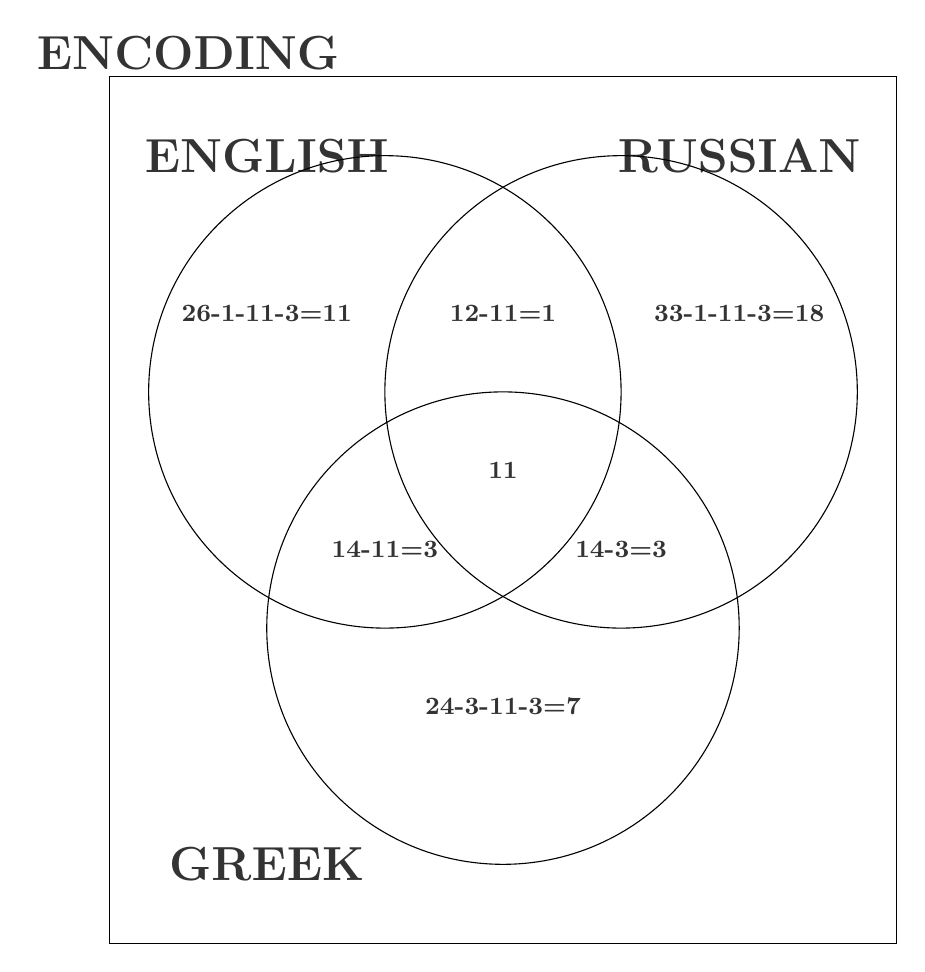
\begin{tikzpicture}
    \begin{scope} [fill opacity = .8]
        \draw (-5,5) rectangle (5,-6);
        \draw[draw = black] (-1.5,1) circle (3);
        \draw[draw = black] (1.5,1) circle (3);
        \draw[draw = black] (0,-2) circle (3);
        \node at (-4,5.3) {\LARGE\textbf{ENCODING}};
        \node at (-3,4) {\LARGE\textbf{ENGLISH}};
        \node at (3,4) {\LARGE\textbf{RUSSIAN}};
        \node at (-3,-5) {\LARGE\textbf{GREEK}};
        \node at (-3,2) {\small\textbf{26-1-11-3=11}};
        \node at (0,2) {\small\textbf{12-11=1}};
        \node at (3,2) {\small\textbf{33-1-11-3=18}};
        \node at (0,0) {\small\textbf{11}};
        \node at (0,-3) {\small\textbf{24-3-11-3=7}};
        \node at (-1.5,-1) {\small\textbf{14-11=3}};
        \node at (1.5,-1) {\small\textbf{14-3=3}};
    \end{scope}
\end{tikzpicture}


Total encodings = 11 + 18 + 7 + 1 + 3 + 3 + 11 = 54 encodings

Therefore, to cover all 54 characters, you would need a UTF-8 encoding with $log_{2} 54 = 6$ x's. 


%444444444444444444444444444444444444444444444444444444444444444444444444444444444444444444444444444444444444444444444444444444444

\newpage
\subsection{Relations}
\subsubsection{Q1}
Let R and S be binary relations on some set A. Prove that if R is antisymmetric then the relation $R\cap S$ must also be antisymmetric.\\
Suppose R is antisymmetric and let $a, b \in A$ such that $aRb$ and $bRa$.\\
\\
Consider:\\
$(a,b)\in R\cap S$ and $(b,a)\in R\cap S$\\
$\Rightarrow (a, b) \in R$ and $(b, a) \in R$, meaning a = b\\
$\therefore$ the elements of $R\cup S$ satisfy a = b.
$\therefore$ if $R$ is antisymmetric then $R\cap S$ must also be antisymmetric.



\subsubsection{Q2}
Let $R = \{(a, b) \in \mathbb{N}^{2}| 3| (a-b)\}$. Prove that R is an equivalence relation.$\\$

To prove that a relation $R$ is an equivalence relation,we need to show three properties — Reflexivity, Symmetry, and Transitivity.$\\$
\textbf{Reflexivity:}
$\forall a \in N$, $3\mid (a-a)$ is always true, since any number minus itself is always zero, and 3 divides 0 evenly.$\\$
\textbf{Symmetry:}\newline
If $(a, b)$ is in $R$, then $3 \mid(a-b)$. This means that $a-b$ is also a multiple of (3).$\\$
Since $(a-b)$ is a multiple of $3,(b-a)$ is also a multiple of $3$ (because if $x$ is a multiple of $3$, then $-x$ is also a multiple of $3$ ).
$\\\therefore$ $3 \mid(b-a)$, and $(b,a)$ is in $R$.$\\$
\textbf{Transitivity: }$\\$
If $(a,b)$ is in $R$ and $(b,c)$ is in $R$, then $3 \mid(a-b)$ and $3 \mid(b-c)$.
By the properties of divisibility, it can be concluded that $3 \mid[(a-b)+(b-c)]$, which is equal to $3 \mid(a-c)$.
Therefore, $(a,c)$ is in $R$.

Since $R$ satisfies all three properties (reflexivity, symmetry, and transitivity), it is an equivalence relation.$\\$
$\therefore$ $R$ is an equivalence relation.



\subsubsection{Q3}
\begin{proof}
Let $A = \{1, 2, 3, 4, 5\}$ and B = \{red, yellow, blue, green, purple\}. Prove that if $f : A \rightarrow B$
is one-to-one then f must also be onto. [Hint: Try a contradiction].\newline
Let $f:A\rightarrow B$ be one-to-one and that $f:A \rightarrow B$ is not onto for the sake of contradiction.\newline
This means that $f(a_{1})=f(a_{2})$ $\rightarrow a_{1}=a_{2}$ and that there is an arbitrary element $b \in B$ that there is no $a\in A$ for some $f(a)=b\\$
Consider, $f(a_{1}) = f(a_{2}) = b\\$
Since $f$ is one-to-one: $f(a_{1}) = f(a_{2}) \Rightarrow a_{1} = a_{2}.\\$
However, this is a contradiction to $b$ not having an $a$ that $f(a)=b\\$
$\therefore$ When $f$ is one-to-one, it must also be onto. $\rightline{Q.E.D.}$
\end{proof}
\subsubsection{Q4}
We can define the relation $\le$ as the following “a $\le$ b if there exists $k \in \mathbb{N}$ such that
a + k = b” (note that k must be greater than zero). Use this definition to prove that $\le$ is
a partial order
\textbf{This question is not done because 5/6 questions have been done}
\subsubsection{Q5}
Let $E$ be the set of all even integers that is $E = \{n|n = 2k \textrm{for some} k \in Z\}$. Let $f : E \rightarrow Z$ be the function $f(x)=\frac{3x-4}{2}$. (a) Is $f$ one to one? (b) Is $f$ onto? (c) If neither is true, give a new domain or co-domain so that the function is a bijection; Otherwise give the inverse$\\$
$n=2k\\$
$f:E\rightarrow Z \Rightarrow f:$even integers $\rightarrow$ integers

(a) Is $f$ one-to-one
Let $x_{1},x_{2} \in E s.t. f(x_{1}) = f(x_{2})\\$
Consider $f(x_{1}) = f(x_{2})\\$
$\frac{3\cdot x_{1}-4}{2} = \frac{3\cdot x_{2}-4}{2}\\$
$2\cdot \frac{3\cdot x_{1}-4}{2} = 2\cdot \frac{3\cdot x_{2}-4}{2}\\$
$3\cdot x_{1}-4 = 3\cdot x_{2}-4\\$
$3\cdot x_{1}-4+4 = 3\cdot x_{2}-4+4\\$
$3\cdot x_{1} = 3\cdot x_{2}\\$
$\frac{3\cdot x_{1}}{3} = \frac{3\cdot x_{2}}{3}\\$
$x_{1}=x_{2}\\$
$\therefore$ when $f(x_{1})=f(x_{2})$ it must be the case that $x_{1}=x_{2}$ so $f$ is one-to-one


(b) Is $f$ onto
Consider the inverse $x=\frac{2\cdot y +4}{3}$ and evaluate$\\$
$f(\frac{2x+4}{3})=\frac{3\cdot \frac{2x+4}{3}-4}{2}$
$=\frac{2y+4-4}{2}\\$
$\frac{2y}{2}\\$
$=y\\$
\underline{WTS}\newline
$y=\frac{3x-4}{2}\\$
$2y=3x+4\\$
$2y-4=3x$
$\frac{2y+4}{3}=x$


Onto means $\forall b \in \mathbb{Z} \exists a\in E s.t. f(a) = b.$ This means that for the formula. for any integer value put in as $y$, it will yield an even integer
$\\\underline{Odd Numbers:} \;\; y=2n+1\\$
$x=\frac{2(2n+1)+4}{3}\\$
$x=\frac{4n+2+4}{3}\\$
$x=\frac{2(xn+2)}{3};$ let $m=2k+2;m\in \mathbb{Z}\\$
$x=\frac{2m}{3}$
$x \neq even\\\\$
$\\\underline{Even Numbers:}\;\; y=2n\\$
$x = \frac{2(2n)+4}{3}\\$
$x = \frac{4n+4}{3}\\$
$x = \frac{2(2n+2)}{3};$ let $m=2n+2;\, m\in \mathbb(R) \\$
$x=\frac{2m}{m}\\$
$x \neq even$
$\therefore\;\;f$ is not onto for the specified co-domain
$\\\\$(c) If neither is true, give a new domain or co-domain so that the function is a bijection; Otherwise give the inverse
$\\$Restrict the range to $3q+1$ for some $q\in \mathbb{Z}\\$
Let $L$ be the set $\{n|n=3q+1 \textrm{ for some }q\in \mathbb{Z}\}\\$
$\therefore f: E \rightarrow L$

\subsubsection{Q6}
Given the recurrence relation $a_{n} = 10a_{n-1} - 31a_{n-2} + 30a_{n-3}$ with $a_{0} = 3$ and $a_{1} = 6$ and
$a_{2} = 6$. Prove using strong induction that the closed form is$\\$ 
$$a_{n} = 3 \cdot 3^{n} - 5^{n} + 2^{n}$$
\newline 
Base Case:$\\$

\begin{table}[ht]
    \centering
    \begin{tabular}{|c|c|c|}
         \hline &  Recursive& Closed\\
         \hline $n=0$&  $a_{0}=3$& $a_{0}=3\cdot 3^{0}-5^{0}+2^{0} $\\
         &  & $=3\cdot 1 - 1 + 1$\\
         &  & $=3-1+1$\\
         &  & $=3$\\
         \hline $n=1$&  $a_{1}=6$& $a_{1}=3\cdot 3^{1}-5^{1}+2^{1} $\\
 & &$=3\cdot 3 - 5 + 2$\\
 & &$=9-3$\\
 & &$=6$\\
 \hline $n=2$& $a_{2}=6$&$a_{2}=3\cdot 3^{2}-5^{2}+2^{2} $\\
 & &$=3\cdot 9 - 25 + 4$\\
 & &$=27-16$\\
 & &$=6$\\
 \hline
    \end{tabular}

\end{table}
$\\ \therefore$ The Base Case Holds$\\$
Induction Hypothesis:$\\$
$a_{j}=3\cdot 2^{j}-5^{j}+2^{j}\\$
Induction Step:$\\$
Consider the Recursive Form $k+1\\$
$a_{k+1}=10a_{(k+1)-1}-31a_{(k+1)-2}+30a_{(k+1)-3}\\$
$=10a_{k}-31a_{k-1}+30a_{k-2}$
$=10(3\cdot 3^{k}-5^{k}+2^{k})-31(3\cdot 3^{k-1}-5^{k-1}+2^{k-1}+30(3\cdot 3^{k-2}-5^{k-2}+2^{k-2})\\$
$=30\cdot 3^{k}-10\cdot 5^{k} +10\cdot 2^{k}-93\cdot 3^{k-1}+31\cdot5^{k-1}-31\cdot 2^{k-1}+90\cdot 3^{k-2}-30\cdot 5^{k-2}+30\cdot 2^{k-2}\\$
$=30\cdot3^{k}-93\cdot3^{k-1}+90\cdot3^{k-2}-10\cdot5^{k}-31\cdot5^{k-1}-30\cdot5^{k-2}+10\cdot2^{k}-31\cdot2^{k-1}+30\cdot^{k-2}\\$
$=3^{k-2}(30\cdot3^{2}-93\cdot3+90)-5^{k-2}(10\cdot5^{2}-31\cdot5+30)+2^{k-2}(10\cdot2^{2}-31\cdot2+30)\\$
$=3^{k-2}(81)-5^{k-2}(125)+2^{k-2}(8)\\$
$=3\cdot3^{k-2}(3^{3})-5^{k-2}(5^{3})+2^{k-2}(2^{3})\\$
\underline{WTS}$\\$
$9_{k+1}=3\cdot3^{k+1}-5^{k+1}+2^{k+1}$
$\\ \therefore$ We have proved by strong induction that the closed form of the Recursive Relation is $3\cdot3^{n}-5^{n}+2^{n}$


\end{document}
